% !TEX TS-program = pdflatex
% !TEX encoding = UTF-8 Unicode
% IEEE Internet of Things Magazine template (IEEEmiot.cls), special issue
% "Digital Service Loops for IoT-Enabled Connected Healthcare Systems".
\documentclass[journal,twoside,web]{IEEEmiot}
\usepackage{cite}
\usepackage{amsmath,amssymb,amsfonts}
\usepackage{graphicx}
\usepackage[mathlines,switch]{lineno}
\usepackage{multicol,multirow}
\usepackage{marginnote}
\usepackage{stfloats}
\usepackage{booktabs}
\usepackage{tikz}
\usetikzlibrary{positioning,calc,arrows.meta,shapes.symbols,shapes.geometric,decorations.pathreplacing}

\usepackage{mcomstd}

\usepackage{hyperref}
\hypersetup{colorlinks,
      linkcolor=nblue,
      citecolor=nblue,
      urlcolor=nblue,
      filecolor=nblue}

\usepackage{etoolbox}

\markboth{\bf VERIFIABLE DIGITAL SERVICE LOOPS}{}

\title{VeriLoop: Verifiable Digital Service Loops\\ for IoT-Enabled Remote Patient Monitoring}

% TODO(authors): names, IEEE membership grades and ORCIDs.
\author{{First A. Author, Second B. Author, and Third C. Author}}

\pubid{\begin{tabular}{@{}p{30pc}@{}}\\[-2pt]\multicolumn{1}{c}{2576-3180~\textcopyright~XXXX~IEEE. Applicable Copyright}\\[7pt]\end{tabular}}


\begin{document}

\maketitle

% TODO(authors): funding statement, or delete.
\funding{Funding information to be added by the authors.}

\doi{10.1109/MIOT.XXXX.XXXXXX}
\DCV{XX XXXX XXXX}
\DOP{XX XXXX XXXX}

\begin{firstfootnote}
% TODO(authors): affiliations, postal addresses and e-mail addresses.
First A. Author is with [Department, Institution, City, Country] (e-mail: author@institution.edu).

Second B. Author is with [Department, Institution, City, Country] (e-mail: author@institution.edu).

Third C. Author is with [Department, Institution, City, Country] (e-mail: author@institution.edu).

The simulator, code and raw results supporting this article are available from the authors (repository link to be added).
\end{firstfootnote}

\bodyfont

\begin{abstract}
Remote patient monitoring has made it cheap to collect vital signs at home, but most deployments still stop at an alert:
nobody checks whether the data behind the alert were trustworthy, whether the action that followed actually helped, or
what the system should learn from the outcome. This article argues that connected healthcare needs \emph{verifiable
digital service loops} in which sensing, interpretation, decision, execution and validation form one closed and
auditable cycle. We present VeriLoop, an edge--fog--cloud architecture that (i) diagnoses sensor faults and confirms
suspicious data with the patient before involving clinicians, (ii) maps risk to a tiered service contract bounded by
National Early Warning Score~2 (NEWS2) red-flag guardrails, (iii) verifies the physiological outcome of every clinical
action and escalates when recovery is not observed, (iv) adapts per-patient operating rules only within clinically
approved bounds, and (v) records every loop iteration in a hash-chained provenance ledger anchored in the cloud. In a
reproducible simulation of 150 virtual patients monitored at home for one week under five random seeds (750 patient-weeks), with injected sensor faults and
connectivity outages, VeriLoop let 5.7\% of deterioration episodes reach a critical state, compared with 18.6\% for
continuous NEWS2 monitoring and 11.7\% for an open-loop machine-learning monitor. It also cut false alarms by 38\% and
60\% respectively, and used 59\% less uplink bandwidth than continuous streaming. Removing outcome verification alone
nearly doubled the adverse-event rate. We release the simulator and code, and close with the governance and
regulatory questions that adaptive, closed-loop health services raise.
\end{abstract}

\section{Introduction}

Internet of Things (IoT) devices now measure heart rate, respiratory rate, oxygen saturation, blood pressure and
temperature at home, and remote patient monitoring (RPM) is routine in chronic and post-discharge
care~\cite{islam2015,farahani2018}. Yet most RPM deployments are still device-centric: data flow from a wearable to a
cloud dashboard, a threshold or early-warning score raises an alert, and the loop ends. Three questions stay
unanswered. Was the alert caused by the patient or the sensor? Did the action that followed work? What should the
system change for this patient? Without answers, RPM services generate alarm fatigue~\cite{sendelbach2013} and cannot
produce the evidence that payers and regulators expect.

This special issue frames the alternative as a \emph{digital service loop}: sensing, interpretation, decision,
execution and validation, with execution outcomes feeding back into the rules. The idea resembles the MAPE-K loop of
autonomic computing~\cite{kephart2003}, but healthcare adds constraints: actions are carried out by people, errors cause
clinical harm, adaptation must stay within limits a clinician can sign off, and every step must be auditable. We
contribute (i) a definition of a \emph{verifiable} service loop whose validation stage confirms data, verifies
outcomes and adapts rules within bounds; (ii) VeriLoop, an edge--fog--cloud realisation with NEWS2
guardrails~\cite{rcp2017}, a hash-chained ledger and an HL7 FHIR mapping~\cite{fhir}; and (iii) an open closed-loop
simulator in which we compare VeriLoop with common designs and ablate each stage.

\section{Why Monitoring Pipelines Are Not Loops}

IoT health systems typically combine body-worn sensors, a smart edge gateway and cloud
analytics~\cite{hassanalieragh2015,rahmani2018}; edge processing cuts bandwidth and latency and survives backhaul
failures~\cite{shi2016}. NEWS2 remains the clinical reference score: each vital sign scores 0--3, and an aggregate of 5,
or any single 3, triggers urgent review~\cite{rcp2017,smith2013}. Machine-learning models increasingly sit on
top~\cite{rajkomar2019}. Seen as a loop, these pipelines are open in three places. \textbf{Data are not validated}:
signal-quality indices~\cite{orphanidou2015} discard bad samples but rarely ask the patient to re-measure or re-seat a
probe. \textbf{Outcomes are not verified}: after an alert, a fixed cooldown suppresses further alarms, so a failed
intervention is noticed only when the cooldown expires. \textbf{Rules either never learn or learn without limits},
raising concerns about software that changes after approval~\cite{fda2021}. Tamper-evident
logging~\cite{haber1991,azaria2016} is feasible but rarely built into the loop itself.
Table~\ref{tab:gap} summarises which loop stages each family of designs closes.

\begin{table}[!t]
\centering
\caption{Loop stages closed by common RPM designs ($\checkmark$ closed, $\circ$ partial, -- open).}
\label{tab:gap}
\footnotesize
\setlength{\tabcolsep}{3pt}
\begin{tabular}{@{}lcccc@{}}
\toprule
Stage & Spot & Cont. & Open-loop & \textbf{Veri-} \\
 & NEWS2 & NEWS2 & ML & \textbf{Loop} \\
\midrule
Continuous sensing & -- & $\checkmark$ & $\checkmark$ & $\checkmark$ \\
Personalised interpretation & -- & -- & $\checkmark$ & $\checkmark$ \\
Fault diagnosis & -- & $\circ$ & $\circ$ & $\checkmark$ \\
Data confirmation with patient & -- & -- & -- & $\checkmark$ \\
Tiered, deadline-tracked actions & $\circ$ & -- & -- & $\checkmark$ \\
Outcome verification & -- & -- & -- & $\checkmark$ \\
Bounded rule adaptation & -- & -- & -- & $\checkmark$ \\
Edge operation during outages & $\checkmark$ & $\circ$ & -- & $\checkmark$ \\
Tamper-evident provenance & -- & -- & -- & $\checkmark$ \\
\bottomrule
\end{tabular}
\end{table}

\section{The VeriLoop Architecture}

Fig.~\ref{fig:arch} shows the deployment and the loop. A home edge gateway runs one loop iteration per sample.

\begin{figure*}[t]
\centering
\resizebox{\textwidth}{!}{% Fig. 1: VeriLoop overview — (a) deployment view, (b) the verifiable service loop.
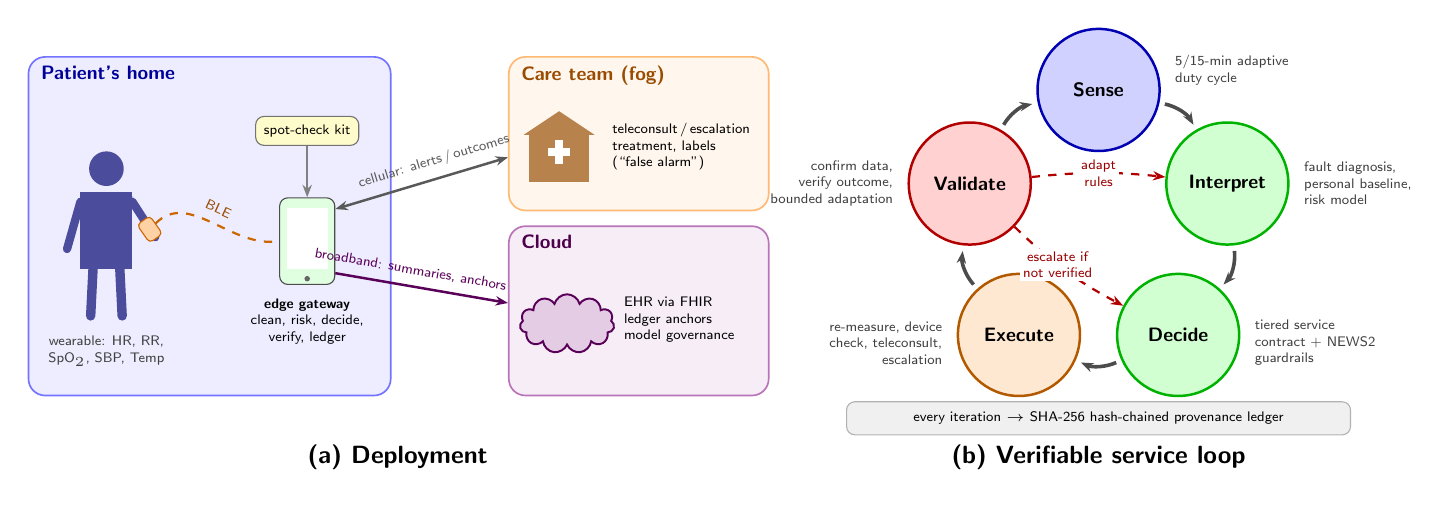
\begin{tikzpicture}[
  font=\sffamily\scriptsize,
  >={Stealth[length=4.5pt]},
  zone/.style={rounded corners=6pt, draw=#1!55, fill=#1!7, line width=0.6pt},
  ztitle/.style={font=\sffamily\scriptsize\bfseries, text=#1!60!black},
  box/.style={rounded corners=3pt, draw=black!55, fill=white, align=center, inner sep=3pt},
  link/.style={->, line width=0.9pt, black!65},
  stage/.style={circle, draw=#1!70!black, fill=#1!18, line width=0.9pt, minimum size=1.55cm, align=center,
                inner sep=0pt, font=\sffamily\scriptsize},
  fb/.style={->, thick, red!70!black, dashed},
  fbl/.style={font=\sffamily\tiny, text=red!60!black, fill=white, inner sep=1pt, align=center},
]
% ====================================================================== (a)
\begin{scope}
\node[zone=blue, minimum width=4.6cm, minimum height=4.3cm, anchor=north west] (home) at (0,0) {};
\node[ztitle=blue, anchor=north west] at (home.north west) {\,Patient's home};
% person
\begin{scope}[shift={(1.0,-2.15)}]
  \fill[blue!45!black!70] (0,0.72) circle (0.22);
  \fill[blue!45!black!70] (-0.33,-0.55) rectangle (0.33,0.42);
  \fill[blue!45!black!70, rounded corners=2pt] (-0.33,0.42) -- (0.33,0.42) -- (0.33,0.3) -- (-0.33,0.3) -- cycle;
  \draw[blue!45!black!70, line width=3pt, line cap=round] (0.33,0.3) -- (0.62,-0.15);
  \draw[blue!45!black!70, line width=3pt, line cap=round] (-0.33,0.3) -- (-0.5,-0.3);
  \draw[blue!45!black!70, line width=3.4pt, line cap=round] (-0.17,-0.55) -- (-0.2,-1.15);
  \draw[blue!45!black!70, line width=3.4pt, line cap=round] (0.17,-0.55) -- (0.2,-1.15);
  % wearable
  \node[draw=orange!80!black, fill=orange!35, rounded corners=1.5pt, minimum width=0.28cm, minimum height=0.2cm,
        inner sep=0pt, rotate=-55] (watch) at (0.55,-0.05) {};
\end{scope}
\node[font=\sffamily\tiny, align=center, text=black!75] at (1.0,-3.75) {wearable: HR, RR,\\SpO$_2$, SBP, Temp};
% gateway (phone)
\node[draw=black!70, fill=green!12, rounded corners=3pt, minimum width=0.7cm, minimum height=1.1cm] (gw) at (3.55,-2.35) {};
\fill[white] ($(gw.center)+(-0.26,-0.36)$) rectangle ($(gw.center)+(0.26,0.42)$);
\fill[black!60] ($(gw.south)+(0,0.08)$) circle (0.035);
\node[font=\sffamily\tiny, align=center, anchor=north] at ($(gw.south)+(0,-0.05)$) {\textbf{edge gateway}\\clean, risk, decide,\\verify, ledger};
\draw[dashed, orange!80!black, thick] (watch) .. controls +(0.5,0.5) and +(-0.6,-0.1) .. node[above, sloped, font=\sffamily\tiny, text=orange!60!black]{BLE} (gw.west);
% spot-check device
\node[box, font=\sffamily\tiny, fill=yellow!20] (spot) at (3.55,-0.95) {spot-check kit};
\end{scope}

% care team (fog)
\begin{scope}[shift={(6.1,0)}]
\node[zone=orange, minimum width=3.3cm, minimum height=1.95cm, anchor=north west] (care) at (0,0) {};
\node[ztitle=orange, anchor=north west] at (care.north west) {\,Care team (fog)};
% clinic icon
\begin{scope}[shift={(0.65,-1.25)}]
  \fill[orange!60!black!70] (-0.38,-0.35) rectangle (0.38,0.25);
  \fill[orange!60!black!70] (-0.45,0.25) -- (0,0.55) -- (0.45,0.25) -- cycle;
  \fill[white] (-0.05,-0.12) rectangle (0.05,0.18);
  \fill[white] (-0.14,-0.02) rectangle (0.14,0.08);
\end{scope}
\node[font=\sffamily\tiny, align=left, anchor=west] at (1.2,-1.15) {teleconsult\,/\,escalation\\treatment, labels\\(``false alarm'')};

\node[zone=violet, minimum width=3.3cm, minimum height=2.15cm, anchor=north west] (cloud) at (0,-2.15) {};
\node[ztitle=violet, anchor=north west] at (cloud.north west) {\,Cloud};
\node[cloud, cloud puffs=11, draw=violet!70!black, fill=violet!20, minimum width=1.2cm, minimum height=0.75cm,
      line width=0.7pt] at (0.75,-3.4) {};
\node[font=\sffamily\tiny, align=left, anchor=west] at (1.35,-3.35) {EHR via FHIR\\ledger anchors\\model governance};
\end{scope}

\draw[link, <->] ($(gw.north east)+(0,-0.15)$) -- node[above, sloped, font=\sffamily\tiny, pos=0.6]{cellular: alerts\,/\,outcomes} ($(care.west)+(0,-0.3)$);
\draw[link, violet!70!black] ($(gw.south east)+(0,0.15)$) -- node[above, sloped, font=\sffamily\tiny, pos=0.42]{broadband: summaries, anchors} ($(cloud.west)+(0,0.1)$);
\draw[link, black!50] (spot.south) -- (gw.north);
\node[font=\sffamily\bfseries\small] at (4.7,-5.1) {(a) Deployment};

% ====================================================================== (b)
\begin{scope}[shift={(13.6,-2.15)}]
\def\R{1.72}
\node[stage=blue]   (s1) at (90:\R)   {\textbf{Sense}};
\node[stage=green]  (s2) at (18:\R)   {\textbf{Interpret}};
\node[stage=green]  (s3) at (-54:\R)  {\textbf{Decide}};
\node[stage=orange] (s4) at (-126:\R) {\textbf{Execute}};
\node[stage=red]    (s5) at (162:\R)  {\textbf{Validate}};
\foreach \a/\b in {s1/s2, s2/s3, s3/s4, s4/s5, s5/s1}
  \draw[->, line width=1.3pt, black!70, shorten >=2pt, shorten <=2pt] (\a) to[bend left=24] (\b);
% feedback chords from Validate
\draw[fb] (s5) to[bend right=8] node[fbl, pos=0.42]{escalate if\\not verified} (s3);
\draw[fb] (s5) to[bend left=6] node[fbl, pos=0.5]{adapt\\rules} (s2);
% stage annotations outside the wheel
\node[font=\sffamily\tiny, align=left, anchor=west, text=black!75] at ($(s1)+(0.85,0.25)$) {5/15-min adaptive\\duty cycle};
\node[font=\sffamily\tiny, align=left, anchor=west, text=black!75] at ($(s2)+(0.85,0)$) {fault diagnosis,\\personal baseline,\\risk model};
\node[font=\sffamily\tiny, align=left, anchor=west, text=black!75] at ($(s3)+(0.85,-0.1)$) {tiered service\\contract + NEWS2\\guardrails};
\node[font=\sffamily\tiny, align=right, anchor=east, text=black!75] at ($(s4)+(-0.85,-0.1)$) {re-measure, device\\check, teleconsult,\\escalation};
\node[font=\sffamily\tiny, align=right, anchor=east, text=black!75] at ($(s5)+(-0.85,0)$) {confirm data,\\verify outcome,\\bounded adaptation};
% ledger bar
\node[draw=gray!60, fill=gray!12, rounded corners=3pt, minimum width=6.4cm, minimum height=0.42cm,
      font=\sffamily\tiny, align=center] at (0,-2.45) {every iteration $\rightarrow$ SHA-256 hash-chained provenance ledger};
\node[font=\sffamily\bfseries\small] at (0,-2.95) {(b) Verifiable service loop};
\end{scope}
\end{tikzpicture}
}
\caption{VeriLoop at a glance. (a) Deployment: the home edge gateway runs the loop, alerts travel over a cellular
fallback, and only summaries and hourly ledger anchors go over the home broadband. (b) The verifiable service loop:
validation feeds back into decision (escalate when recovery is not verified) and interpretation (bounded adaptation),
and every iteration is written to a hash-chained provenance ledger.}
\label{fig:arch}
\end{figure*}

\textbf{Sense.} The wearable samples every 15 minutes while the patient is stable and every 5 minutes once risk rises.

\textbf{Interpret.} The edge rejects implausible values, holds back sudden jumps until the next sample confirms them
(removing motion spikes), flags frozen channels, and marks an isolated SpO$_2$ or blood-pressure deviation that no other
vital sign corroborates as \emph{suspect}. A logistic-regression risk model turns 16 features (deviation from a 24-hour
personal baseline, one-hour mean and 30-minute trend per vital sign, plus NEWS2) into a risk score. We chose an
inspectable model whose coefficients a clinician can review.

\textbf{Decide.} A tiered service contract maps risk to actions: Tier~0 routine summaries; Tier~1 patient or device
requests (re-measure, re-seat a sensor); Tier~2 teleconsultation when personal risk or NEWS2 reaches amber for two
samples; Tier~3 escalation at NEWS2 $\geq 7$ or very high risk. Every Tier~2 trigger, and every Tier~3 trigger resting
on one vital sign, is first confirmed by a Tier~1 re-measurement; an unanswered request escalates anyway. NEWS2 red flags
are guardrails that adaptation can never relax.

\textbf{Execute.} Requests are tracked as open service requests with deadlines. Alerts use a cellular fallback, so a
broadband outage delays only routine uploads.

\textbf{Validate.} Validation has three jobs. \emph{Confirm the data}: if a re-measurement contradicts the wearable, the
trigger is cancelled and a device check is requested. \emph{Verify the outcome}: 90 minutes after treatment starts,
VeriLoop escalates if neither risk nor NEWS2 has fallen. \emph{Adapt within bounds}: after a clinician-labelled false
alarm, the patient's risk threshold rises by 0.05 (cap 0.85), the NEWS2 amber threshold may rise from 5 to 6, and the
baseline is refreshed; this is the kind of pre-declared change envelope regulators ask of adaptive
software~\cite{fda2021}. Fig.~\ref{fig:lifecycle} follows one request through these steps.

\begin{figure*}[t]
\centering
\resizebox{\textwidth}{!}{% Fig. 2: lifecycle of one verified service request (swimlane / sequence view)
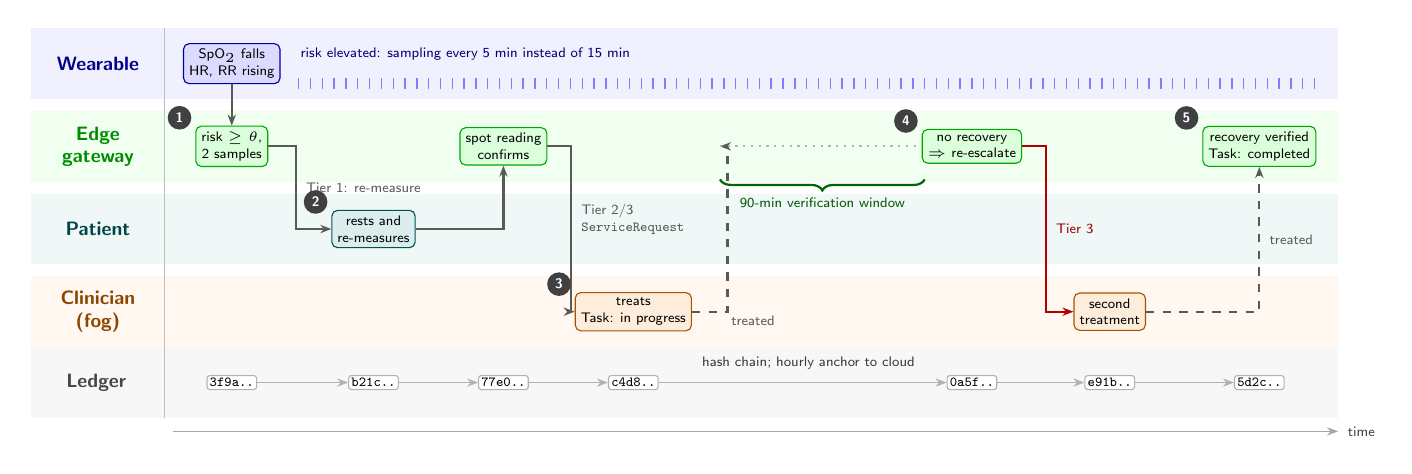
\begin{tikzpicture}[
  font=\sffamily\scriptsize,
  >={Stealth[length=4pt]},
  lane/.style={fill=#1!6, draw=none},
  lname/.style={font=\sffamily\scriptsize\bfseries, text=#1!55!black, align=center, text width=1.55cm},
  ev/.style={rounded corners=2pt, draw=#1!65!black, fill=#1!14, align=center, inner sep=2pt, font=\sffamily\tiny},
  msg/.style={->, thick, black!65},
  bad/.style={->, thick, red!70!black},
  num/.style={circle, fill=black!75, text=white, font=\sffamily\tiny\bfseries, inner sep=0pt, minimum size=0.3cm},
  hash/.style={draw=gray!60, fill=white, font=\ttfamily\tiny, inner sep=1pt, rounded corners=1pt},
]
\def\W{16.6}
% lanes (y positions)
\def\yW{0} \def\yE{-1.05} \def\yP{-2.1} \def\yC{-3.15} \def\yL{-4.05}
\foreach \y/\c/\n in {\yW/blue/Wearable, \yE/green/Edge gateway, \yP/teal/Patient, \yC/orange/Clinician (fog), \yL/gray/Ledger\,/\,cloud}{
  \fill[lane=\c] (0,\y-0.45) rectangle (\W,\y+0.45);
  \node[lname=\c] at (0.85,\y) {\n};
}
\draw[gray!50] (1.7,0.45) -- (1.7,\yL-0.45);
% time axis
\draw[->, gray!70] (1.8,\yL-0.62) -- (\W,\yL-0.62) node[right, font=\sffamily\tiny, text=gray!50!black]{time};

% 1: anomaly
\node[ev=blue] (a1) at (2.55,\yW) {SpO$_2$ falls\\HR, RR rising};
\node[ev=green] (b1) at (2.55,\yE) {risk $\geq\theta$,\\2 samples};
\draw[msg] (a1) -- (b1);
\node[num] at ($(b1.north west)+(-0.2,0.1)$) {1};
% 2: confirm with patient
\node[ev=teal] (p1) at (4.35,\yP) {rests and\\re-measures};
\draw[msg] (b1.east) -- ++(0.35,0) |- node[pos=0.25, right, font=\sffamily\tiny]{Tier 1: re-measure} (p1.west);
\node[ev=green] (b2) at (6.0,\yE) {spot reading\\confirms};
\draw[msg] (p1.east) -| (b2.south);
\node[num] at ($(p1.north west)+(-0.2,0.1)$) {2};
% 3: escalate
\node[ev=orange] (c1) at (7.65,\yC) {treats\\Task: in progress};
\draw[msg] (b2.east) -- ++(0.3,0) |- node[pos=0.22, right, font=\sffamily\tiny, align=left]{Tier 2/3\\\texttt{ServiceRequest}} (c1.west);
\node[num] at ($(c1.north west)+(-0.2,0.1)$) {3};
% 4: verification window
\draw[decorate, decoration={brace, amplitude=4pt, mirror}, thick, green!40!black] (8.75,\yE-0.42) -- node[below=3pt, font=\sffamily\tiny, text=green!35!black]{90-min verification window} (11.35,\yE-0.42);
\node[ev=green] (b3) at (11.95,\yE) {no recovery\\$\Rightarrow$ re-escalate};
\draw[msg, dashed] (c1.east) -- ++(0.45,0) node[below right, font=\sffamily\tiny, inner sep=1pt]{treated} |- (8.75,\yE);
\draw[gray!60, dotted, thick] (8.75,\yE) -- (b3.west);
\node[num] at ($(b3.north west)+(-0.2,0.1)$) {4};
\node[ev=orange] (c2) at (13.7,\yC) {second\\treatment};
\draw[bad] (b3.east) -- ++(0.3,0) |- node[pos=0.25, right, font=\sffamily\tiny, text=red!60!black]{Tier 3} (c2.west);
\node[ev=green] (b4) at (15.6,\yE) {recovery verified\\Task: completed};
\draw[msg, dashed] (c2.east) -| node[pos=0.75, right, font=\sffamily\tiny]{treated} (b4.south);
\node[num] at ($(b4.north west)+(-0.2,0.1)$) {5};

% sampling ticks on the wearable lane
\foreach \x in {3.4,3.55,...,16.4} \draw[blue!50, line width=0.5pt] (\x,\yW-0.32) -- (\x,\yW-0.18);
\node[font=\sffamily\tiny, text=blue!45!black, anchor=west] at (3.3,\yW+0.12) {risk elevated: sampling every 5 min instead of 15 min};
% ledger: hashes under every step
\foreach \x/\h [count=\i] in {2.55/{3f9a..}, 4.35/{b21c..}, 6.0/{77e0..}, 7.65/{c4d8..}, 11.95/{0a5f..}, 13.7/{e91b..}, 15.6/{5d2c..}}{
  \node[hash] (h\i) at (\x,\yL) {\h};
}
\foreach \a [evaluate=\a as \b using int(\a+1)] in {1,...,6}
  \draw[->, gray!60] (h\a) -- (h\b);
\node[font=\sffamily\tiny, text=gray!45!black, anchor=west] at (8.4,\yL+0.25) {hash chain; hourly anchor to cloud};
\end{tikzpicture}
}
\caption{Lifecycle of one verified service request. (1) The edge detects rising risk and raises the sampling rate.
(2) Before calling a clinician it asks the patient to re-measure. (3) The confirmed reading becomes a Tier~2/3
\texttt{ServiceRequest}, and the clinician starts treatment. (4) Ninety minutes later no recovery is visible, so the
edge escalates again instead of waiting for an alarm cooldown. (5) Recovery after the second treatment is verified and
the \texttt{Task} is closed. Each step adds a link to the hash chain.}
\label{fig:lifecycle}
\end{figure*}

\textbf{Provenance and interoperability.} Each iteration (observation digest, flags, risk, tier, action) is appended to
a SHA-256 hash chain at the edge~\cite{haber1991}, and the chain head is anchored hourly in the cloud, so edits,
reordering or truncation are detectable. Observations map to FHIR \texttt{Observation}, requests to
\texttt{ServiceRequest} and \texttt{Task}, and decisions carry a \texttt{Provenance} resource holding the ledger
hash~\cite{fhir}. A Tier~2 trigger, for example, becomes a \texttt{ServiceRequest} referencing the confirming
\texttt{Observation}s, a \texttt{Task} whose status moves from \emph{requested} to \emph{in-progress} when the clinician
acts and to \emph{completed} only when the verification stage confirms recovery, and a \texttt{Provenance} entry for
each transition. Any FHIR-capable electronic health record can therefore display not only that an alert fired, but
whether the resulting action was carried out and whether it worked.

\section{Evaluation Methodology}

Closed loops need an environment that reacts to alerts, which retrospective datasets cannot provide, so we built a
discrete-event simulator (Fig.~\ref{fig:method}). The results compare designs under identical, controlled conditions
and are not estimates of clinical effect sizes.

\begin{figure*}[t]
\centering
\resizebox{\textwidth}{!}{% Fig. 3: evaluation methodology (closed-loop simulation pipeline)
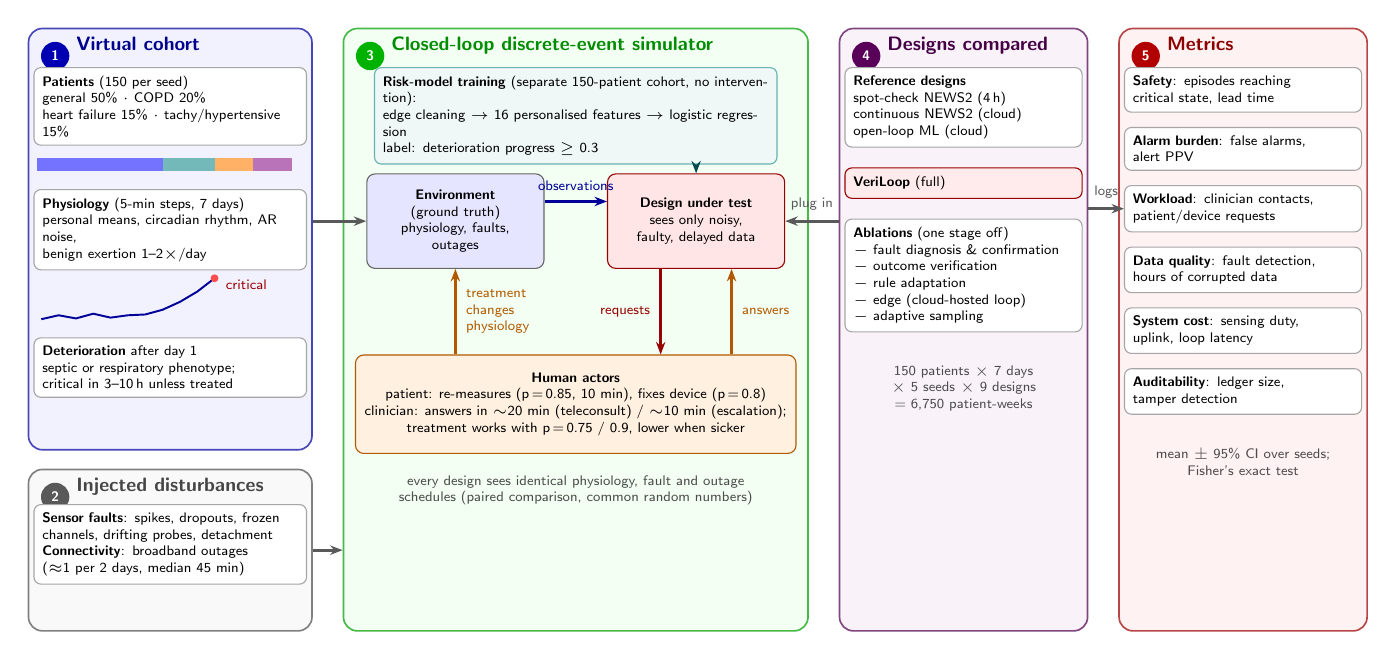
\begin{tikzpicture}[
  font=\sffamily\scriptsize,
  >={Stealth[length=4.5pt]},
  panel/.style={rounded corners=5pt, draw=#1!45!gray, fill=#1!5, line width=0.6pt},
  ptitle/.style={font=\sffamily\scriptsize\bfseries, text=#1!55!black, anchor=north west},
  item/.style={rounded corners=2.5pt, draw=black!35, fill=white, align=left, text width=#1, inner sep=3pt,
               font=\sffamily\tiny},
  it/.style={rounded corners=2.5pt, draw=black!35, fill=white, align=left, inner sep=3pt, font=\sffamily\tiny},
  arr/.style={->, line width=1.1pt, black!65},
  loop/.style={->, line width=1pt, #1},
  badge/.style={circle, fill=#1!70!black, text=white, font=\sffamily\tiny\bfseries, inner sep=1.2pt, minimum size=0.36cm},
]
% ---------------------------------------------------------------- column 1
\node[panel=blue, minimum width=3.6cm, minimum height=5.35cm, anchor=north west] (c1) at (0,0) {};
\node[ptitle=blue] at (c1.north west) {\,\tikz[baseline=-0.6ex]\node[badge=blue]{1};\ Virtual cohort};
\node[it, text width=3.25cm, anchor=north] (g) at ($(c1.north)+(0,-0.5)$)
  {\textbf{Patients} (150 per seed)\\general 50\% $\cdot$ COPD 20\%\\heart failure 15\% $\cdot$ tachy/hypertensive 15\%};
% little population bar
\begin{scope}[shift={($(g.south west)+(0.05,-0.32)$)}]
  \fill[blue!55] (0,0) rectangle (1.6,0.16);
  \fill[teal!55] (1.6,0) rectangle (2.25,0.16);
  \fill[orange!60] (2.25,0) rectangle (2.74,0.16);
  \fill[violet!55] (2.74,0) rectangle (3.23,0.16);
\end{scope}
\node[it, text width=3.25cm, anchor=north] (ph) at ($(g.south)+(0,-0.55)$)
  {\textbf{Physiology} (5-min steps, 7 days)\\personal means, circadian rhythm, AR noise,\\benign exertion 1--2$\times$/day};
% tiny vital-sign sparkline
\draw[blue!60!black, line width=0.7pt] ($(ph.south west)+(0.1,-0.62)$)
   -- ++(0.22,0.05) -- ++(0.22,-0.04) -- ++(0.22,0.06) -- ++(0.22,-0.05) -- ++(0.22,0.03) -- ++(0.22,0.01)
   -- ++(0.22,0.06) -- ++(0.22,0.1) -- ++(0.22,0.13) -- ++(0.22,0.17) coordinate (spk);
\fill[red!70] (spk) circle (0.05);
\node[font=\sffamily\tiny, text=red!60!black, anchor=west] at ($(spk)+(0.02,-0.08)$) {critical};
\node[it, text width=3.25cm, anchor=north] (ep) at ($(ph.south)+(0,-0.85)$)
  {\textbf{Deterioration} after day 1\\septic or respiratory phenotype;\\critical in 3--10\,h unless treated};

% ---------------------------------------------------------------- column 1b: disturbances
\node[panel=gray, minimum width=3.6cm, minimum height=2.05cm, anchor=north west] (c1b) at (0,-5.6) {};
\node[ptitle=gray] at (c1b.north west) {\,\tikz[baseline=-0.6ex]\node[badge=gray]{2};\ Injected disturbances};
\node[it, text width=3.25cm, anchor=north] at ($(c1b.north)+(0,-0.45)$)
  {\textbf{Sensor faults}: spikes, dropouts, frozen\\channels, drifting probes, detachment\\\textbf{Connectivity}: broadband outages\\($\approx$1 per 2 days, median 45 min)};

% ---------------------------------------------------------------- column 2: simulator
\node[panel=green, minimum width=5.9cm, minimum height=7.65cm, anchor=north west] (c2) at (4.0,0) {};
\node[ptitle=green] at (c2.north west) {\,\tikz[baseline=-0.6ex]\node[badge=green]{3};\ Closed-loop discrete-event simulator};
% training box at top
\node[item=4.9cm, draw=teal!60, fill=teal!6, anchor=north] (train) at ($(c2.north)+(0,-0.5)$)
  {\textbf{Risk-model training} (separate 150-patient cohort, no intervention):\\edge cleaning $\rightarrow$ 16 personalised features $\rightarrow$ logistic regression\\label: deterioration progress $\geq$ 0.3};
\node[rounded corners=3pt, draw=black!60, fill=blue!10, minimum width=2.25cm, minimum height=1.2cm, align=center,
      font=\sffamily\tiny, anchor=north west] (env) at ($(c2.north west)+(0.3,-1.85)$)
  {\textbf{Environment}\\(ground truth)\\physiology, faults,\\outages};
\node[rounded corners=3pt, draw=red!60!black, fill=red!10, minimum width=2.25cm, minimum height=1.2cm, align=center,
      font=\sffamily\tiny, anchor=north east] (dut) at ($(c2.north east)+(-0.3,-1.85)$)
  {\textbf{Design under test}\\sees only noisy,\\faulty, delayed data};
\node[rounded corners=3pt, draw=orange!70!black, fill=orange!12, minimum width=5.3cm, minimum height=1.25cm, align=center,
      font=\sffamily\tiny, anchor=north] (hum) at ($(c2.north)+(0,-4.15)$)
  {\textbf{Human actors}\\patient: re-measures (p\,=\,0.85, 10 min), fixes device (p\,=\,0.8)\\clinician: answers in $\sim$20 min (teleconsult) / $\sim$10 min (escalation);\\treatment works with p\,=\,0.75 / 0.9, lower when sicker};
\draw[loop=blue!60!black] ($(env.east)+(0,0.25)$) -- node[above, font=\sffamily\tiny]{observations} ($(dut.west)+(0,0.25)$);
\coordinate (rq1) at ($(dut.south)+(-0.45,0)$);
\coordinate (an1) at ($(dut.south)+(0.45,0)$);
\draw[loop=red!60!black] (rq1) -- node[left, font=\sffamily\tiny]{requests} (rq1 |- hum.north);
\draw[loop=orange!70!black] (an1 |- hum.north) -- node[right, font=\sffamily\tiny]{answers} (an1);
\draw[loop=orange!70!black] (hum.north -| env.south) -- node[right, font=\sffamily\tiny, align=left]{treatment\\changes\\physiology} (env.south);
\draw[arr, teal!60!black] (train.south -| dut.north) -- (dut.north);
\node[font=\sffamily\tiny, align=center, text=black!70, anchor=north] at ($(hum.south)+(0,-0.15)$)
  {every design sees identical physiology, fault and outage\\schedules (paired comparison, common random numbers)};

% ---------------------------------------------------------------- column 3: designs
\node[panel=violet, minimum width=3.15cm, minimum height=7.65cm, anchor=north west] (c3) at (10.3,0) {};
\node[ptitle=violet] at (c3.north west) {\,\tikz[baseline=-0.6ex]\node[badge=violet]{4};\ Designs compared};
\node[it, text width=2.8cm, anchor=north] (ref) at ($(c3.north)+(0,-0.5)$)
  {\textbf{Reference designs}\\spot-check NEWS2 (4\,h)\\continuous NEWS2 (cloud)\\open-loop ML (cloud)};
\node[it, text width=2.8cm, anchor=north, draw=red!60!black, fill=red!8] (vl) at ($(ref.south)+(0,-0.25)$)
  {\textbf{VeriLoop} (full)};
\node[it, text width=2.8cm, anchor=north] (abl) at ($(vl.south)+(0,-0.25)$)
  {\textbf{Ablations} (one stage off)\\$-$ fault diagnosis \& confirmation\\$-$ outcome verification\\$-$ rule adaptation\\$-$ edge (cloud-hosted loop)\\$-$ adaptive sampling};
\node[font=\sffamily\tiny, align=center, text=black!70, anchor=north] at ($(abl.south)+(0,-0.3)$)
  {150 patients $\times$ 7 days\\$\times$ 5 seeds $\times$ 9 designs\\= 6{,}750 patient-weeks};

% ---------------------------------------------------------------- column 4: metrics
\node[panel=red, minimum width=3.15cm, minimum height=7.65cm, anchor=north west] (c4) at (13.85,0) {};
\node[ptitle=red] at (c4.north west) {\,\tikz[baseline=-0.6ex]\node[badge=red]{5};\ Metrics};
\node[it, text width=2.8cm, anchor=north] (m1) at ($(c4.north)+(0,-0.5)$) {\textbf{Safety}: episodes reaching\\critical state, lead time};
\node[it, text width=2.8cm, anchor=north] (m2) at ($(m1.south)+(0,-0.18)$) {\textbf{Alarm burden}: false alarms,\\alert PPV};
\node[it, text width=2.8cm, anchor=north] (m3) at ($(m2.south)+(0,-0.18)$) {\textbf{Workload}: clinician contacts,\\patient/device requests};
\node[it, text width=2.8cm, anchor=north] (m4) at ($(m3.south)+(0,-0.18)$) {\textbf{Data quality}: fault detection,\\hours of corrupted data};
\node[it, text width=2.8cm, anchor=north] (m5) at ($(m4.south)+(0,-0.18)$) {\textbf{System cost}: sensing duty,\\uplink, loop latency};
\node[it, text width=2.8cm, anchor=north] (m6) at ($(m5.south)+(0,-0.18)$) {\textbf{Auditability}: ledger size,\\tamper detection};
\node[font=\sffamily\tiny, align=center, text=black!70, anchor=north] at ($(m6.south)+(0,-0.3)$) {mean $\pm$ 95\% CI over seeds;\\Fisher's exact test};

% ---------------------------------------------------------------- flow arrows between columns
\draw[arr] (c1.east |- env.west) ++(0,0) -- (env.west);
\draw[arr] (c1b.east) -- (c1b.east -| c2.west);
\draw[arr] (c3.west |- dut.east) -- node[above, font=\sffamily\tiny]{plug in} (dut.east);
\draw[arr] (c3.east |- m3.west) -- node[above, font=\sffamily\tiny]{logs} (m3.west);
\end{tikzpicture}
}
\caption{Evaluation methodology. A virtual cohort (1) and injected sensor faults and outages (2) drive a closed-loop
simulator (3) in which the design under test sees only what a real deployment would see, and its requests are answered
by simulated patients and clinicians whose treatments change the physiology. Every design (4) runs on identical
schedules, and the logs are scored on six groups of metrics (5).}
\label{fig:method}
\end{figure*}

Patients come from four sub-groups (general, COPD on NEWS2 SpO$_2$ scale~2, heart failure, tachycardic/hypertensive)
with personal baselines, circadian rhythm, noise and daily exertion. About 40\% develop septic or respiratory
deterioration that becomes critical in 3--10 hours unless effectively treated; reaching that state counts as an adverse
event. Devices suffer spikes, dropouts, frozen channels, drifting probes and detachment, and home broadband fails about
every two days. Simulated patients answer requests with probability 0.8--0.85; clinicians respond in about 20 minutes
(10 for escalations) and their treatment succeeds with probability 0.75--0.9, less often when the patient is sicker.

We compare \emph{spot-check NEWS2} (one reading every 4 hours), \emph{continuous NEWS2} (5-minute streaming, 10-minute
persistence, 4-hour cooldown), \emph{open-loop ML} (VeriLoop's risk model in the cloud with a fixed threshold and
cooldown) and VeriLoop, plus five ablations. The risk model was trained on a separate simulated cohort (validation AUROC
0.99, reflecting the simulator rather than real-world performance). Each design sees the same 150 patients over seven
days in each of five seeds.

\textbf{Metrics.} We report, per design, the share of deterioration episodes that reach the critical state (the primary
safety outcome), the median lead time between the first alert and that state, false alarms and alert precision,
clinician contacts and patient requests per patient-day, hours spent with corrupted data, sensing duty cycle, uplink
volume and the share of samples whose sense-to-decision latency exceeds one minute. Confidence intervals are 95\%
intervals across seeds; differences in adverse events are tested with Fisher's exact test on pooled episodes, and
paired seed-level comparisons are used for burden metrics.

\section{Results}

Table~\ref{tab:results} summarises all designs; the cohort produced 409 deterioration episodes in 4,500 evaluated
patient-days.

\begin{table*}[t]
\centering
\caption{Results for all designs (mean over five seeds of 150 patients, 409 deterioration episodes; 95\% CI shown for the
primary outcome). Lead time runs from the first clinician alert to the point at which the untreated episode would become
critical. ``Corrupted data'' is hours per patient-day with at least one faulty channel; ``late'' is the share of samples
processed more than one minute after sensing.}
\label{tab:results}
\footnotesize\setlength{\tabcolsep}{3.6pt}
\resizebox{\textwidth}{!}{%
\begin{tabular}{lcccccccccc}
\toprule
 & \multicolumn{2}{c}{Safety} & \multicolumn{2}{c}{Alarm burden} & \multicolumn{2}{c}{Workload (/patient-day)} &
 Data quality & \multicolumn{3}{c}{System cost} \\
\cmidrule(lr){2-3}\cmidrule(lr){4-5}\cmidrule(lr){6-7}\cmidrule(lr){8-8}\cmidrule(lr){9-11}
Design & \shortstack{Critical\\(\%)} & \shortstack{Lead\\(h)} & \shortstack{False alarms\\/patient-day} &
\shortstack{PPV\\(\%)} & \shortstack{Clinician\\contacts} & \shortstack{Patient\\requests} &
\shortstack{Corrupted\\data (h/pd)} & \shortstack{Sensing\\duty (\%)} & \shortstack{Uplink\\(KB/pd)} &
\shortstack{Late\\(\%)} \\
\midrule
% rows generated by code/make_figures.py -> figures/table_combined.tex
\multicolumn{11}{l}{\textit{Reference designs}} \\
Spot-check NEWS2 (4 h) & 64.5\,$\pm$\,4.0 & 1.7 & 0.37 & 16 & 0.50 & 0.0 & 4.3 & 2 & 0.6 & 1.8 \\
Continuous NEWS2 & 18.6\,$\pm$\,6.0 & 2.9 & 0.96 & 14 & 1.28 & 0.0 & 4.3 & 100 & 28.1 & 1.9 \\
Open-loop ML (cloud) & 11.7\,$\pm$\,3.9 & 4.6 & 1.49 & 11 & 1.84 & 0.0 & 4.3 & 100 & 28.1 & 1.9 \\
\midrule
\multicolumn{11}{l}{\textit{Proposed}} \\
\textbf{VeriLoop} & 5.7\,$\pm$\,2.5 & 4.3 & 0.59 & 33 & 1.07 & 2.5 & 2.2 & 54 & 11.6 & 0.0 \\
\midrule
\multicolumn{11}{l}{\textit{VeriLoop ablations (one stage removed)}} \\
$-$ fault diagnosis \& confirmation & 5.7\,$\pm$\,2.9 & 4.5 & 1.68 & 16 & 2.20 & 0.0 & 4.3 & 57 & 13.1 & 0.0 \\
$-$ outcome verification & 10.4\,$\pm$\,3.2 & 4.3 & 0.49 & 29 & 0.84 & 2.2 & 2.3 & 54 & 11.6 & 0.0 \\
$-$ rule adaptation & 6.1\,$\pm$\,2.3 & 4.3 & 0.73 & 29 & 1.21 & 2.7 & 2.2 & 55 & 12.2 & 0.0 \\
$-$ edge (cloud-hosted loop) & 5.5\,$\pm$\,1.5 & 4.2 & 0.59 & 33 & 1.09 & 2.5 & 2.3 & 54 & 15.1 & 1.7 \\
$-$ adaptive sampling & 4.5\,$\pm$\,2.3 & 4.3 & 0.73 & 28 & 1.21 & 3.2 & 2.0 & 100 & 12.2 & 0.0 \\
\bottomrule
\end{tabular}}
\end{table*}

\begin{figure*}[!t]
\centering
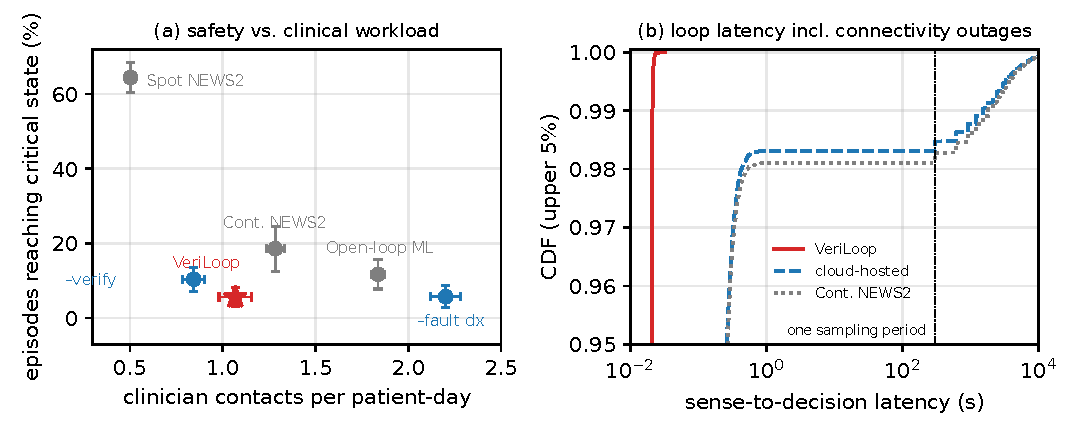
\includegraphics[width=\textwidth]{figures/results.pdf}
\caption{(a) Share of episodes reaching a critical state versus clinician contacts per patient-day (95\% CIs over five
seeds). (b) Upper tail of the sense-to-decision latency distribution. Cloud-hosted designs wait for connectivity
outages to end; the edge loop does not.}
\label{fig:results}
\end{figure*}

\textbf{Safety and alarm burden.} Spot checks missed 28\% of episodes and 64\% became critical. Continuous NEWS2 caught
every episode but late (2.9 hours before the critical point), and 18.6\% became critical. Open-loop ML alerted earlier
(4.6 hours) and reached 11.7\%, but with the most false alarms (1.49 per patient-day). VeriLoop let 5.7\% of episodes
become critical (23 of 409, against 74 for continuous NEWS2, Fisher's exact $p<10^{-7}$, and 47 for open-loop ML,
$p=0.004$) while cutting false alarms by 38\% and 60\%, which doubled alert precision to 33\%. It is the only design in
the low-risk, moderate-workload corner of Fig.~\ref{fig:results}(a). The costs: confirmation takes about 18 minutes of
lead time relative to open-loop ML, and patients receive 2.5 re-measure or device-check requests per day.

\begin{figure}[!t]
\centering
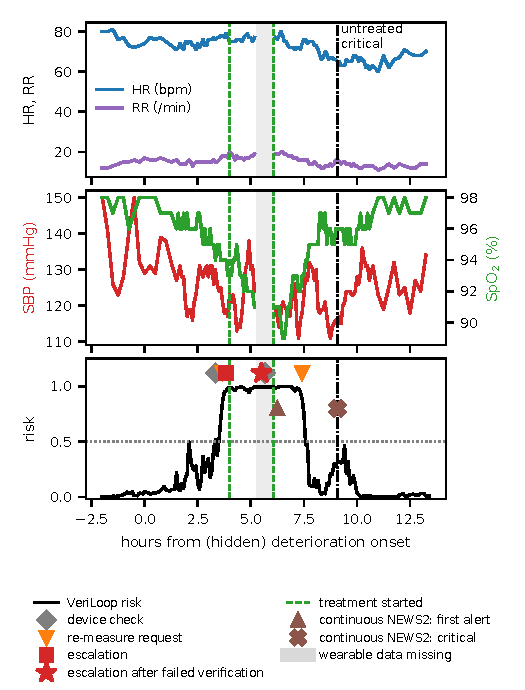
\includegraphics[width=\columnwidth]{figures/case_trace.pdf}
\caption{One simulated loop trace (respiratory deterioration). An early SpO$_2$ fall is first treated as a suspect
reading and checked, then confirmed by re-measurement and escalated. The first treatment fails; outcome verification
detects this 90 minutes later and escalates again, and the second treatment works. Under continuous NEWS2 the same
patient is first alerted 2.4 hours later and reaches the critical state.}
\label{fig:case}
\end{figure}

\textbf{Outcome verification drives most of the safety gain.} Without it, the adverse-event rate rose to 10.4\% (43 of
409, $p=0.014$), because a failed treatment was noticed only when the 4-hour cooldown expired. Fig.~\ref{fig:case} shows the mechanism on one patient: with verification, the failed first treatment is caught 90 minutes after it starts, and the second treatment arrives before the critical state. Verification escalations
were rare (0.07 per patient-day) and 99\% occurred during real episodes, but the full loop needed 0.22 more clinician
contacts per patient-day; intervention-specific verification windows would reduce this.

\textbf{Fault diagnosis halves the noise.} Without it, safety was unchanged but false alarms nearly tripled (1.68 per
patient-day) and clinician contacts doubled. Device-check requests cut time with corrupted data from 4.3 to 2.2 hours per
patient-day. The edge flagged faults with 71\% precision and 69\% recall (range checks alone: 40\% recall); imperfect
precision is why suspect readings are re-measured rather than discarded. In Fig.~\ref{fig:case} a genuine SpO$_2$ fall was first treated as suspect, and only the re-measurement prevented a delay.

\textbf{Adaptation, edge and sampling.} Bounded adaptation removed 19\% of false alarms with no detectable safety
cost. Hosting the loop in the cloud did not change outcomes, because outages are short relative to deterioration, but
1.7\% of samples waited over a minute (99th percentile about 16 minutes versus 21~ms at the edge,
Fig.~\ref{fig:results}(b)) and uplink grew 30\%. Adaptive sampling halved sensing duty without a significant safety
change, and VeriLoop uploaded 11.6~KB per patient-day versus 28.1~KB for streaming.

\textbf{Auditability is cheap.} The ledger stored about 294 entries (44~KB) per patient-day; appending took 1.5~$\mu$s
and verifying a patient-week 2.5~ms. Verification against the hourly anchors detected all 1,000 random modification,
deletion, reordering and truncation attacks; truncation is detectable back to the last anchor.

\section{Lessons and Open Challenges}

\textbf{Validation is a design stage, not a dashboard.} The largest gain came from checking whether an action worked,
which fits the request lifecycle FHIR \texttt{Task} already describes. Every RPM service should state, per action, what
recovery is expected and by when. \textbf{Adaptation needs a declared envelope}: one-directional, capped steps that never
touch red flags turn ``a learning system'' into a reviewable list of permitted changes, and the ledger proves the
envelope was respected~\cite{fda2021}. \textbf{Loops redistribute work}: confirmation shifts effort from clinicians to
patients, so pilots must measure patient burden and adherence.

\textbf{Deployment considerations.} Three practical points follow from building VeriLoop. First, the edge gateway
needs only modest resources: the loop logic, the risk model and the ledger together run in under a millisecond per
sample, so a home hub or a smartphone suffices, and keeping the loop at the edge also keeps raw vital signs at home
unless an action requires them. Second, the tiered contract is a clinical artefact, not a software constant: its tiers,
deadlines, verification windows and adaptation bounds should be agreed with the care team, versioned and stored with
the ledger so that every decision can be traced to the contract in force at the time. Third, the patient is an actor in
the loop, so requests must be clear, few and accessible; patients who cannot re-measure reliably need a carer, a
simpler device or a lower Tier~1 threshold for direct clinician review.

\textbf{Limitations.} All results come from simulation with parameterised physiology, faults and human behaviour, and
the clinician is assumed to recognise apparent deterioration perfectly. Absolute rates are not clinical predictions.
Security was evaluated only for log integrity; confidentiality, device authentication and attacks within an anchor
interval remain open.

\textbf{Open challenges.} The community needs shared closed-loop \emph{benchmarks} calibrated on real RPM cohorts,
\emph{governance} rules for who is accountable when a patient does not act on a request, and \emph{interoperable service
contracts} so tiers, deadlines and verification rules are exchangeable standard resources rather than hard-coded.
Beyond these, closed loops raise new \emph{security} questions: an attacker who can inject a plausible re-measurement
or suppress a verification sample can steer the loop, so device attestation and authenticated patient input become
part of clinical safety, not only of privacy. Finally, \emph{multi-morbidity} complicates verification, because the
expected recovery after an intervention depends on the patient's other conditions and treatments; learning
verification windows per patient, within bounds that clinicians approve, is a natural next step for service loops.

\section{Conclusion}

Device-centric remote monitoring stops at the alert. VeriLoop closes the loop by validating data before acting,
verifying outcomes after acting, adapting only within declared bounds and recording every step in a tamper-evident
ledger. In simulation these mechanisms cut the share of deteriorations reaching a critical state by more than
two-thirds relative to continuous NEWS2 while lowering false alarms, with outcome verification the most important
stage. The next step is calibration on real RPM data and a supervised home-care pilot.



\section{Code and Data Availability}
The simulator, VeriLoop implementation, FHIR mapping, experiment scripts and raw results are provided with this
article (repository link to be added on acceptance), so that every number in Table~\ref{tab:results} can be
regenerated.

\bibliographystyle{IEEEtran}
\bibliography{refs}

\section{Biographies}
\vspace*{-30pt}
% TODO(authors): replace with real biographies (IEEE membership, e-mail, degrees, positions, research interests).
\begin{biographynophoto}
{FIRST A. AUTHOR} (author@institution.edu) is with [Institution]. Biography to be completed.

{SECOND B. AUTHOR} (author@institution.edu) is with [Institution]. Biography to be completed.

{THIRD C. AUTHOR} (author@institution.edu) is with [Institution]. Biography to be completed.
\end{biographynophoto}

\vfill
\end{document}
